\documentclass[a4paper,12pt]{article}
\usepackage[utf8]{inputenc}

\usepackage[top=2cm,bottom=2cm,right=2cm,left=2cm]{geometry}
\usepackage{amsmath,amssymb,enumitem,multicol,graphicx,tikz,framed,tcolorbox,mathtools,comment,subcaption,array,pgfplots}
\usepackage{listings}
\usepackage{xcolor}
\linespread{1.3}
%New colors defined below
\definecolor{codegreen}{rgb}{0,0.6,0}
\definecolor{codegray}{rgb}{0.5,0.5,0.5}
\definecolor{codepurple}{rgb}{0.58,0,0.82}
\definecolor{backcolour}{rgb}{0.95,0.95,0.92}
\setlength\parindent{0pt}
%Code listing style named "mystyle"
\lstdefinestyle{mystyle}{
  backgroundcolor=\color{backcolour},   commentstyle=\color{codegreen},
  keywordstyle=\color{magenta},
  numberstyle=\tiny\color{codegray},
  stringstyle=\color{codepurple},
  basicstyle=\ttfamily\footnotesize,
  breakatwhitespace=false,         
  breaklines=true,                 
  captionpos=b,                    
  keepspaces=true,                 
  numbers=left,                    
  numbersep=5pt,                  
  showspaces=false,                
  showstringspaces=false,
  showtabs=false,                  
  tabsize=2
}

%"mystyle" code listing set
\lstset{style=mystyle}


\usepackage{lipsum,hyperref}
\hypersetup{
	colorlinks=true,
	linkcolor=blue,
	filecolor=magenta,      
	urlcolor=cyan,
}

\begin{document}
\section{Review}
\begin{figure}[!ht]
	\centering
	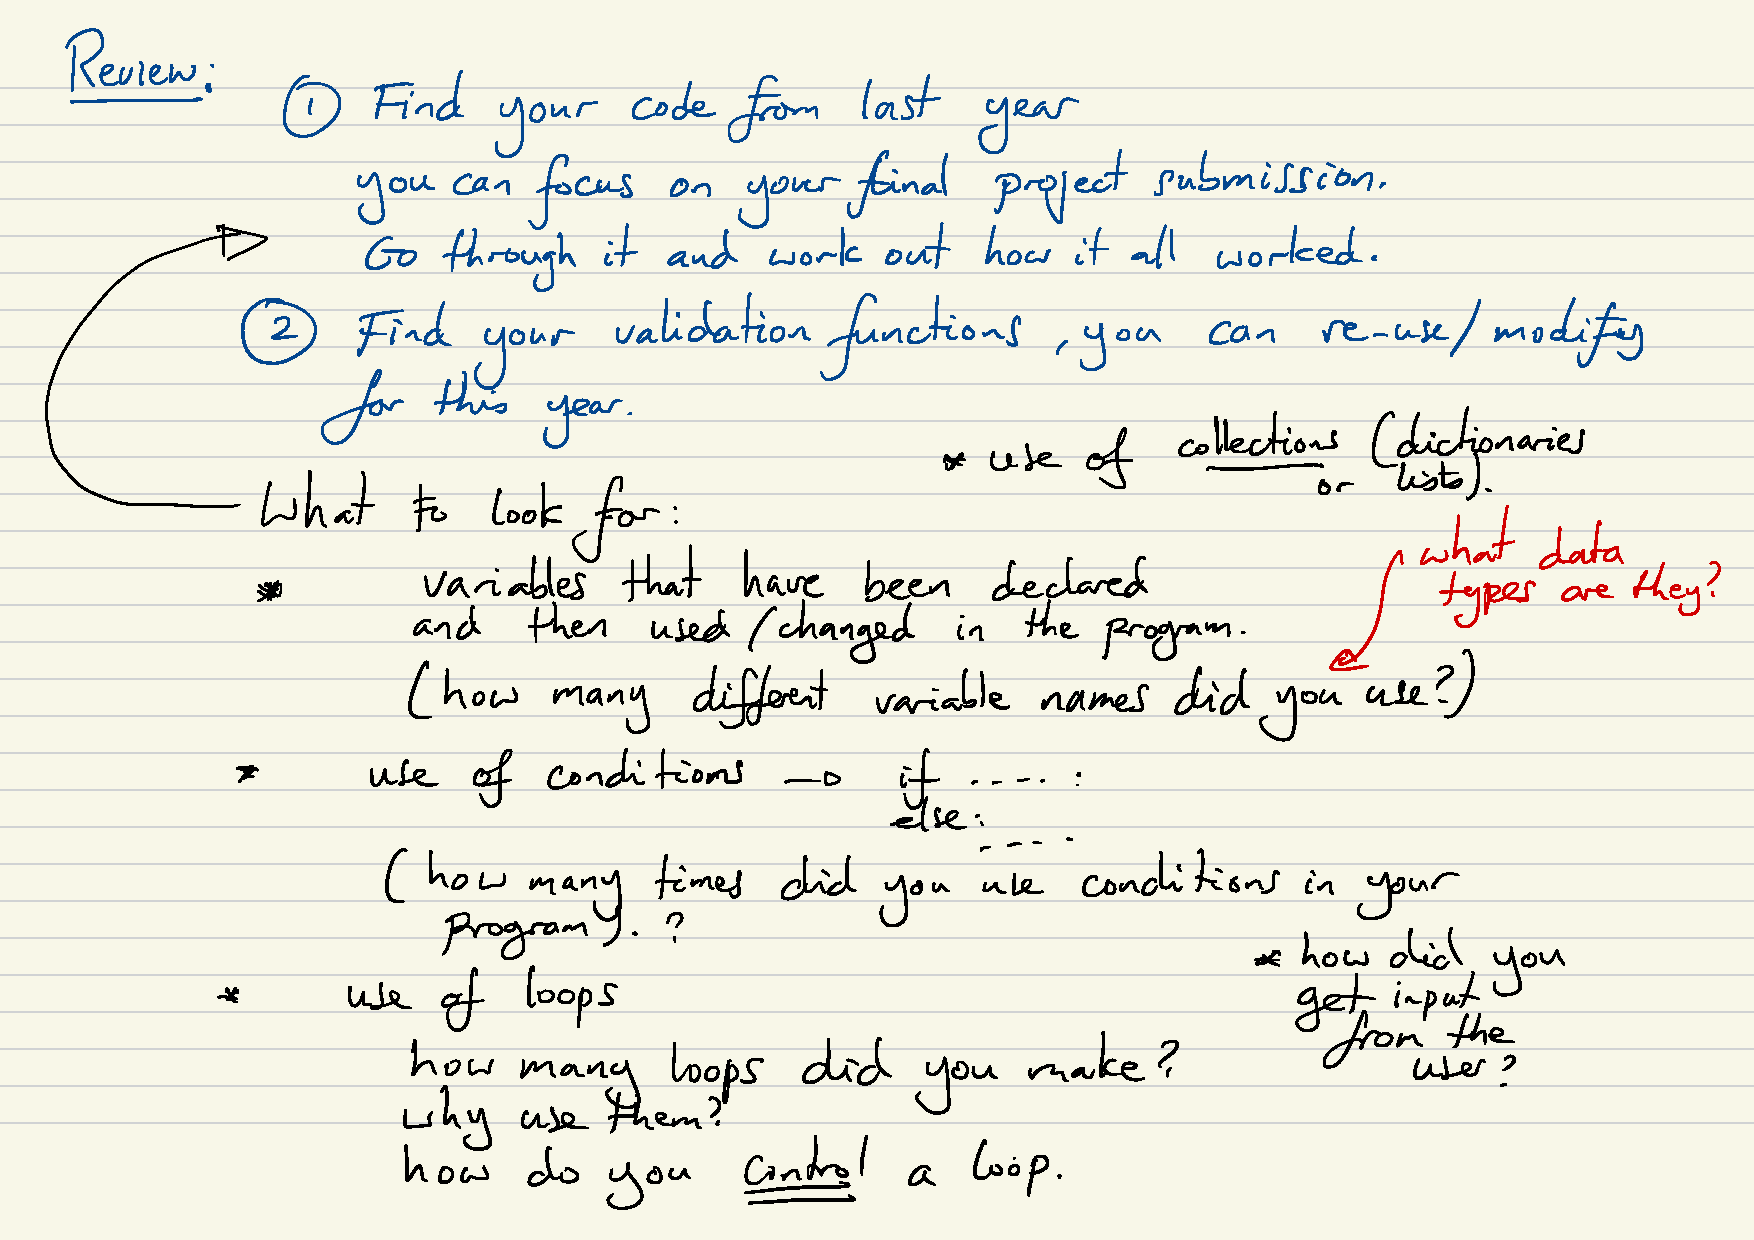
\includegraphics[width=15cm]{review_page.pdf}
\end{figure}
\newpage
\section{Functions}
\begin{figure}[!ht]
	\centering
	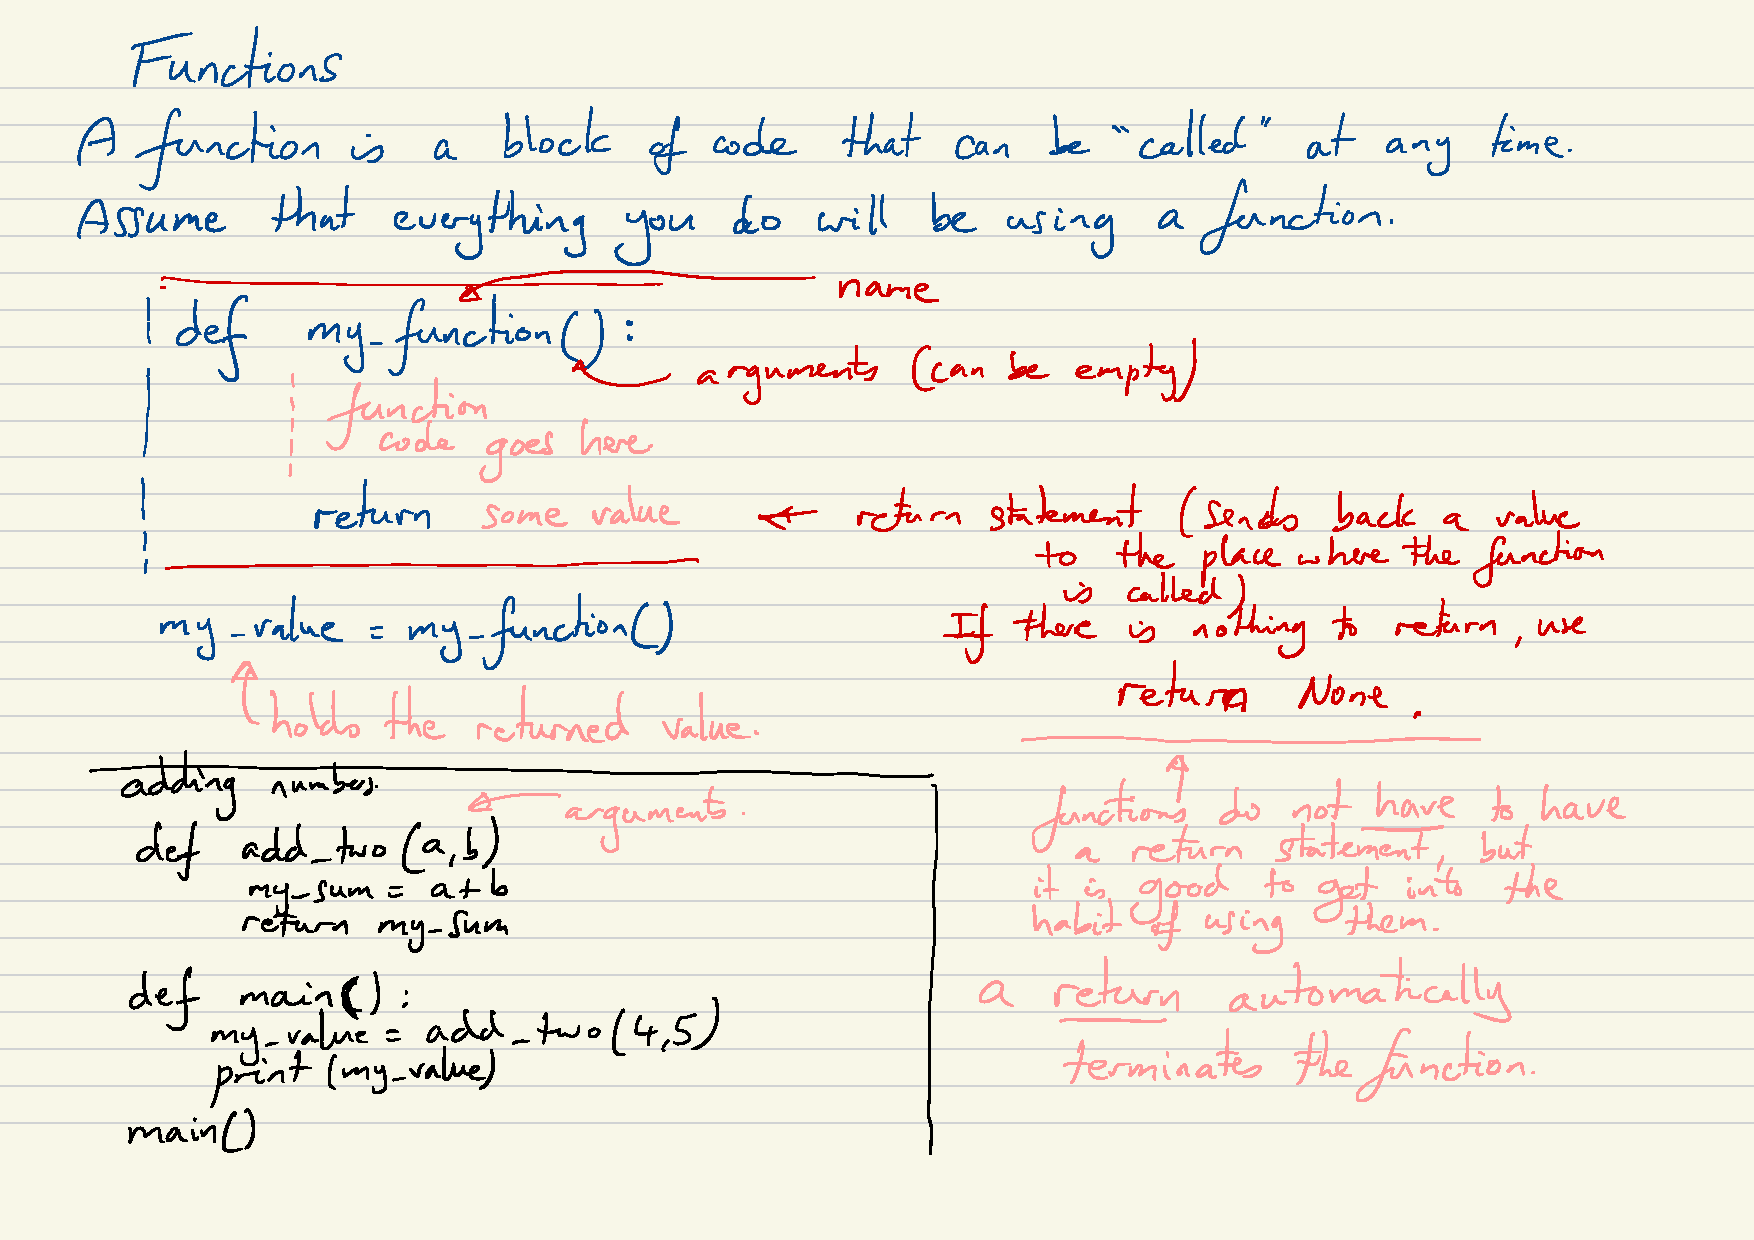
\includegraphics[width=16cm]{functions.pdf}
\end{figure}
\begin{itemize}
\item Functions allow programmers to avoid creating code that has lots of repetitions.
\item Functions allow programmers to break the structure of a program into blocks (or modules), which means that different problems can be separated out and dealt with independently.
\end{itemize}
\lstinputlisting[language=Python, caption = Test program - functions and menu]{py_files/set_two.py}
\newpage

\begin{figure}[!ht]
	\centering
	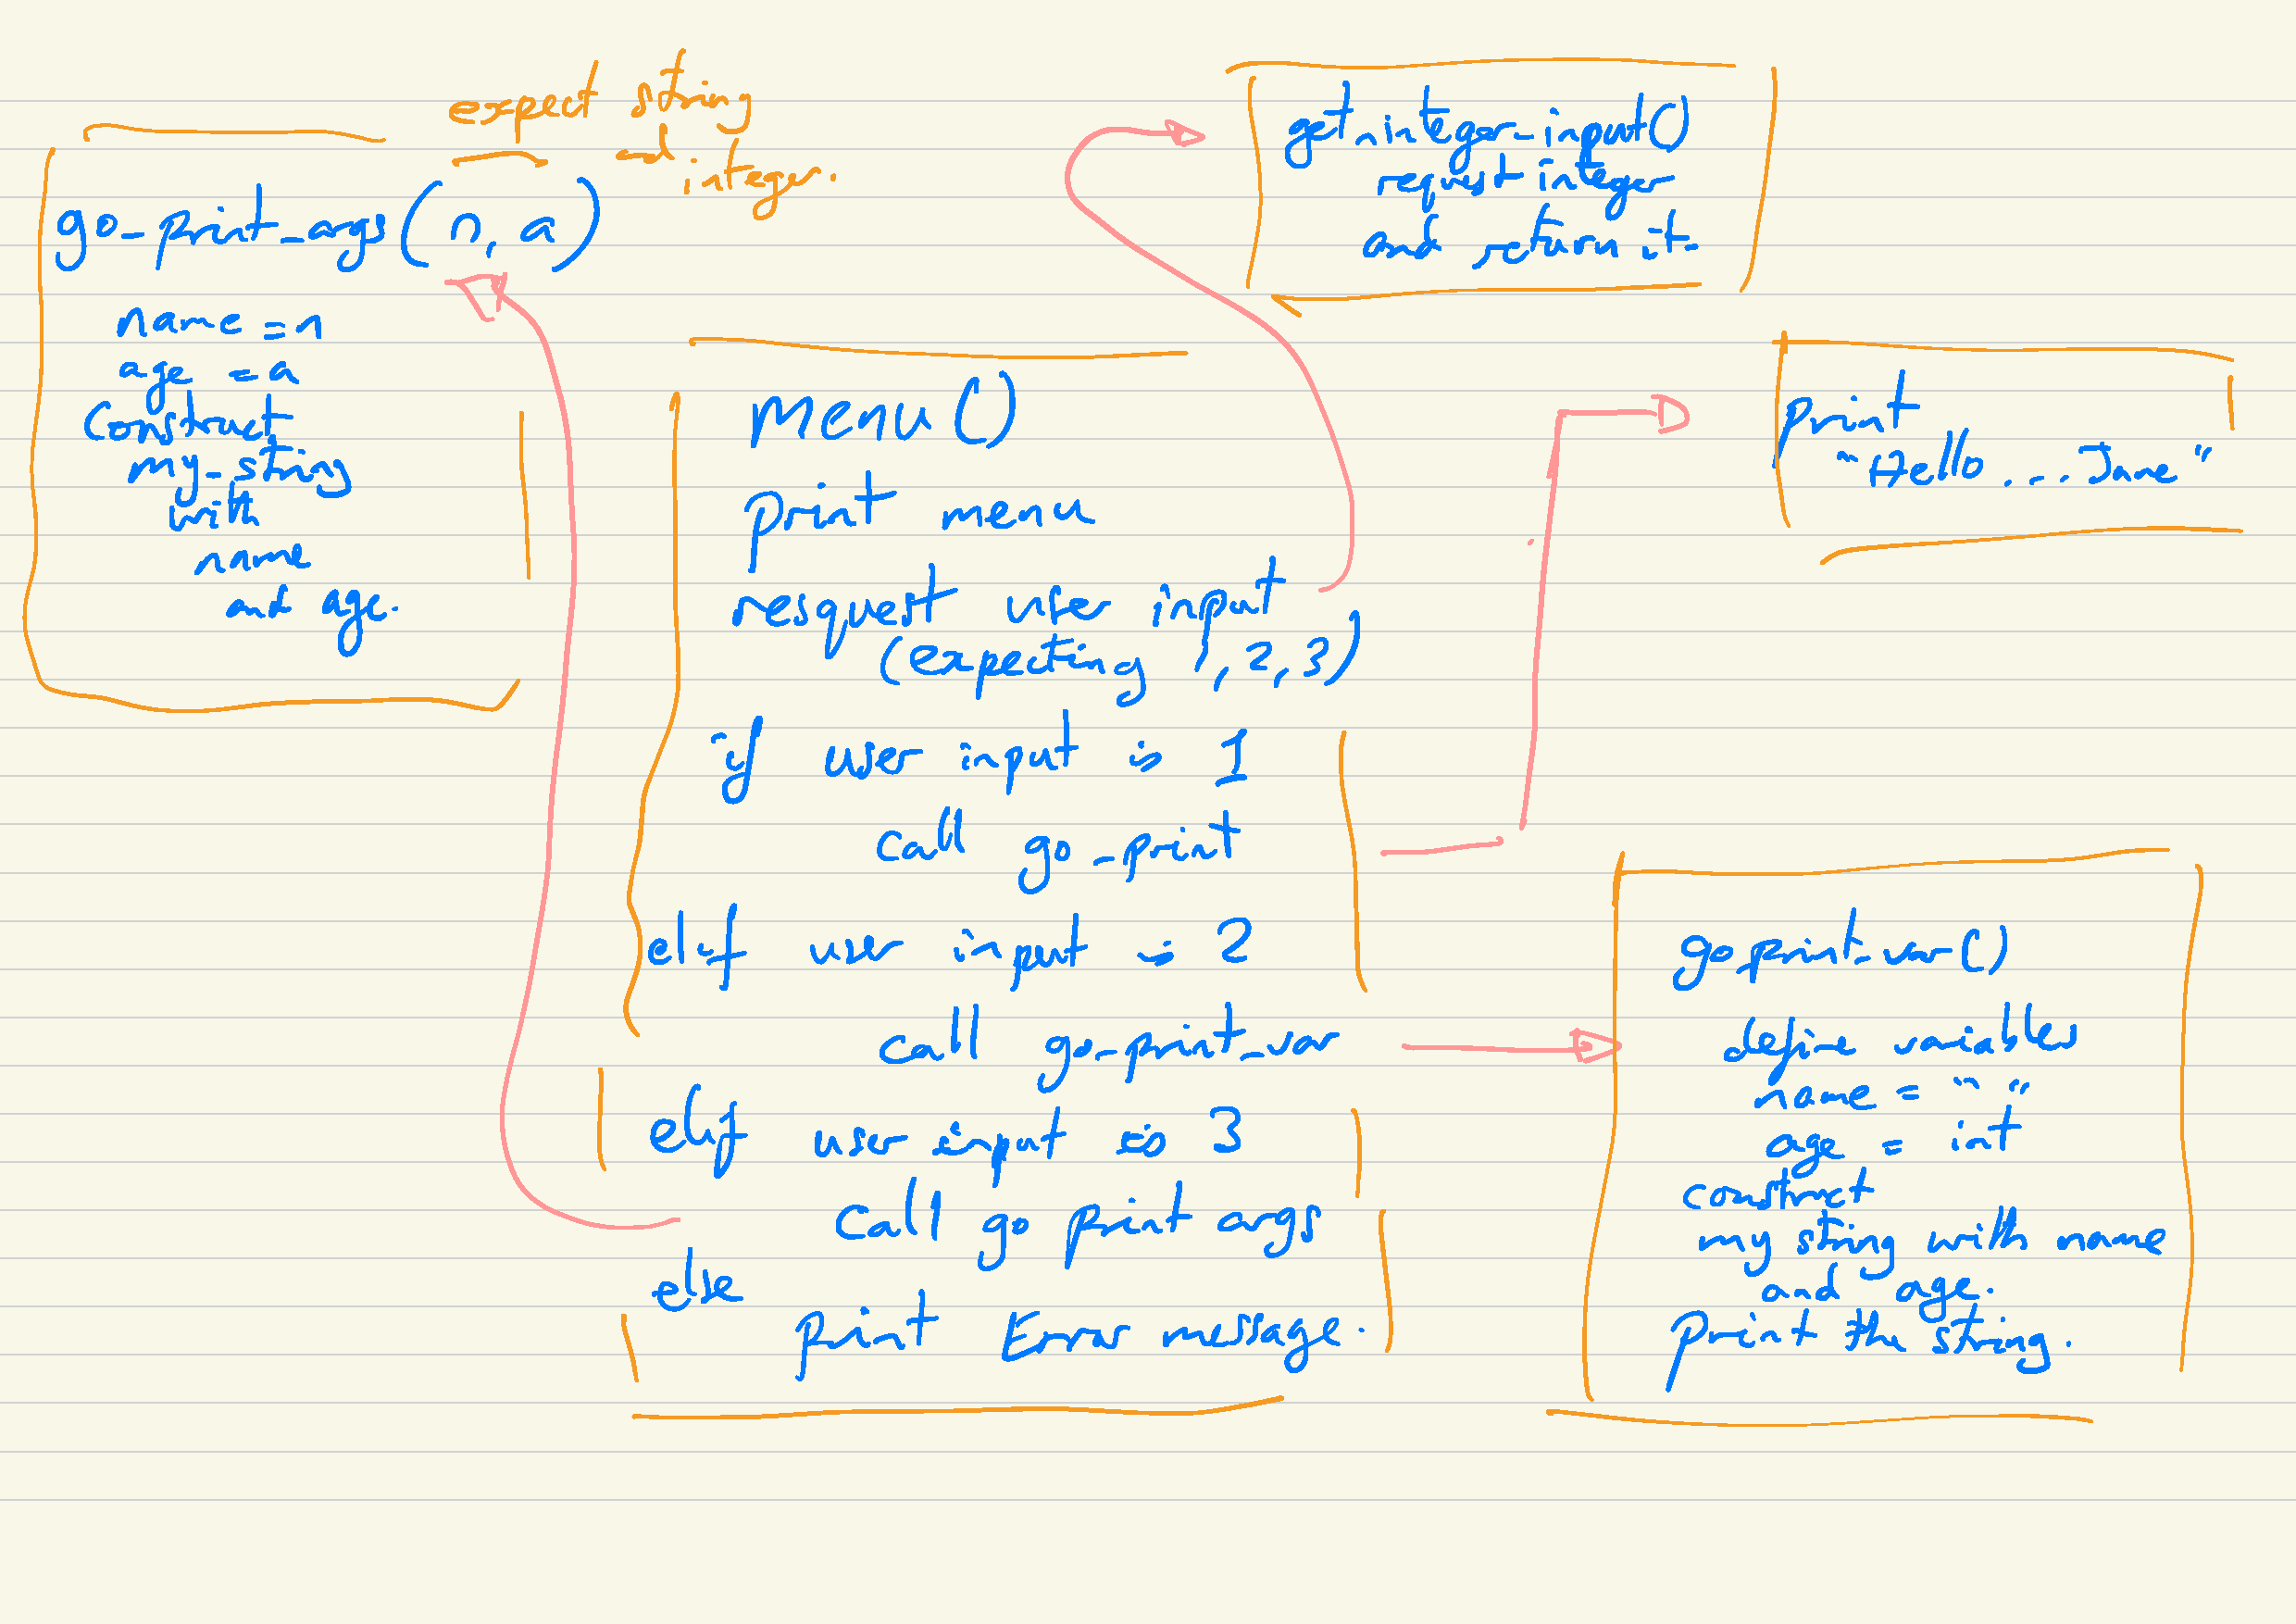
\includegraphics[width=15cm]{function_plan_1.pdf}
	\caption*{Simple Plan}
\end{figure}

\begin{figure}[!ht]
	\centering
	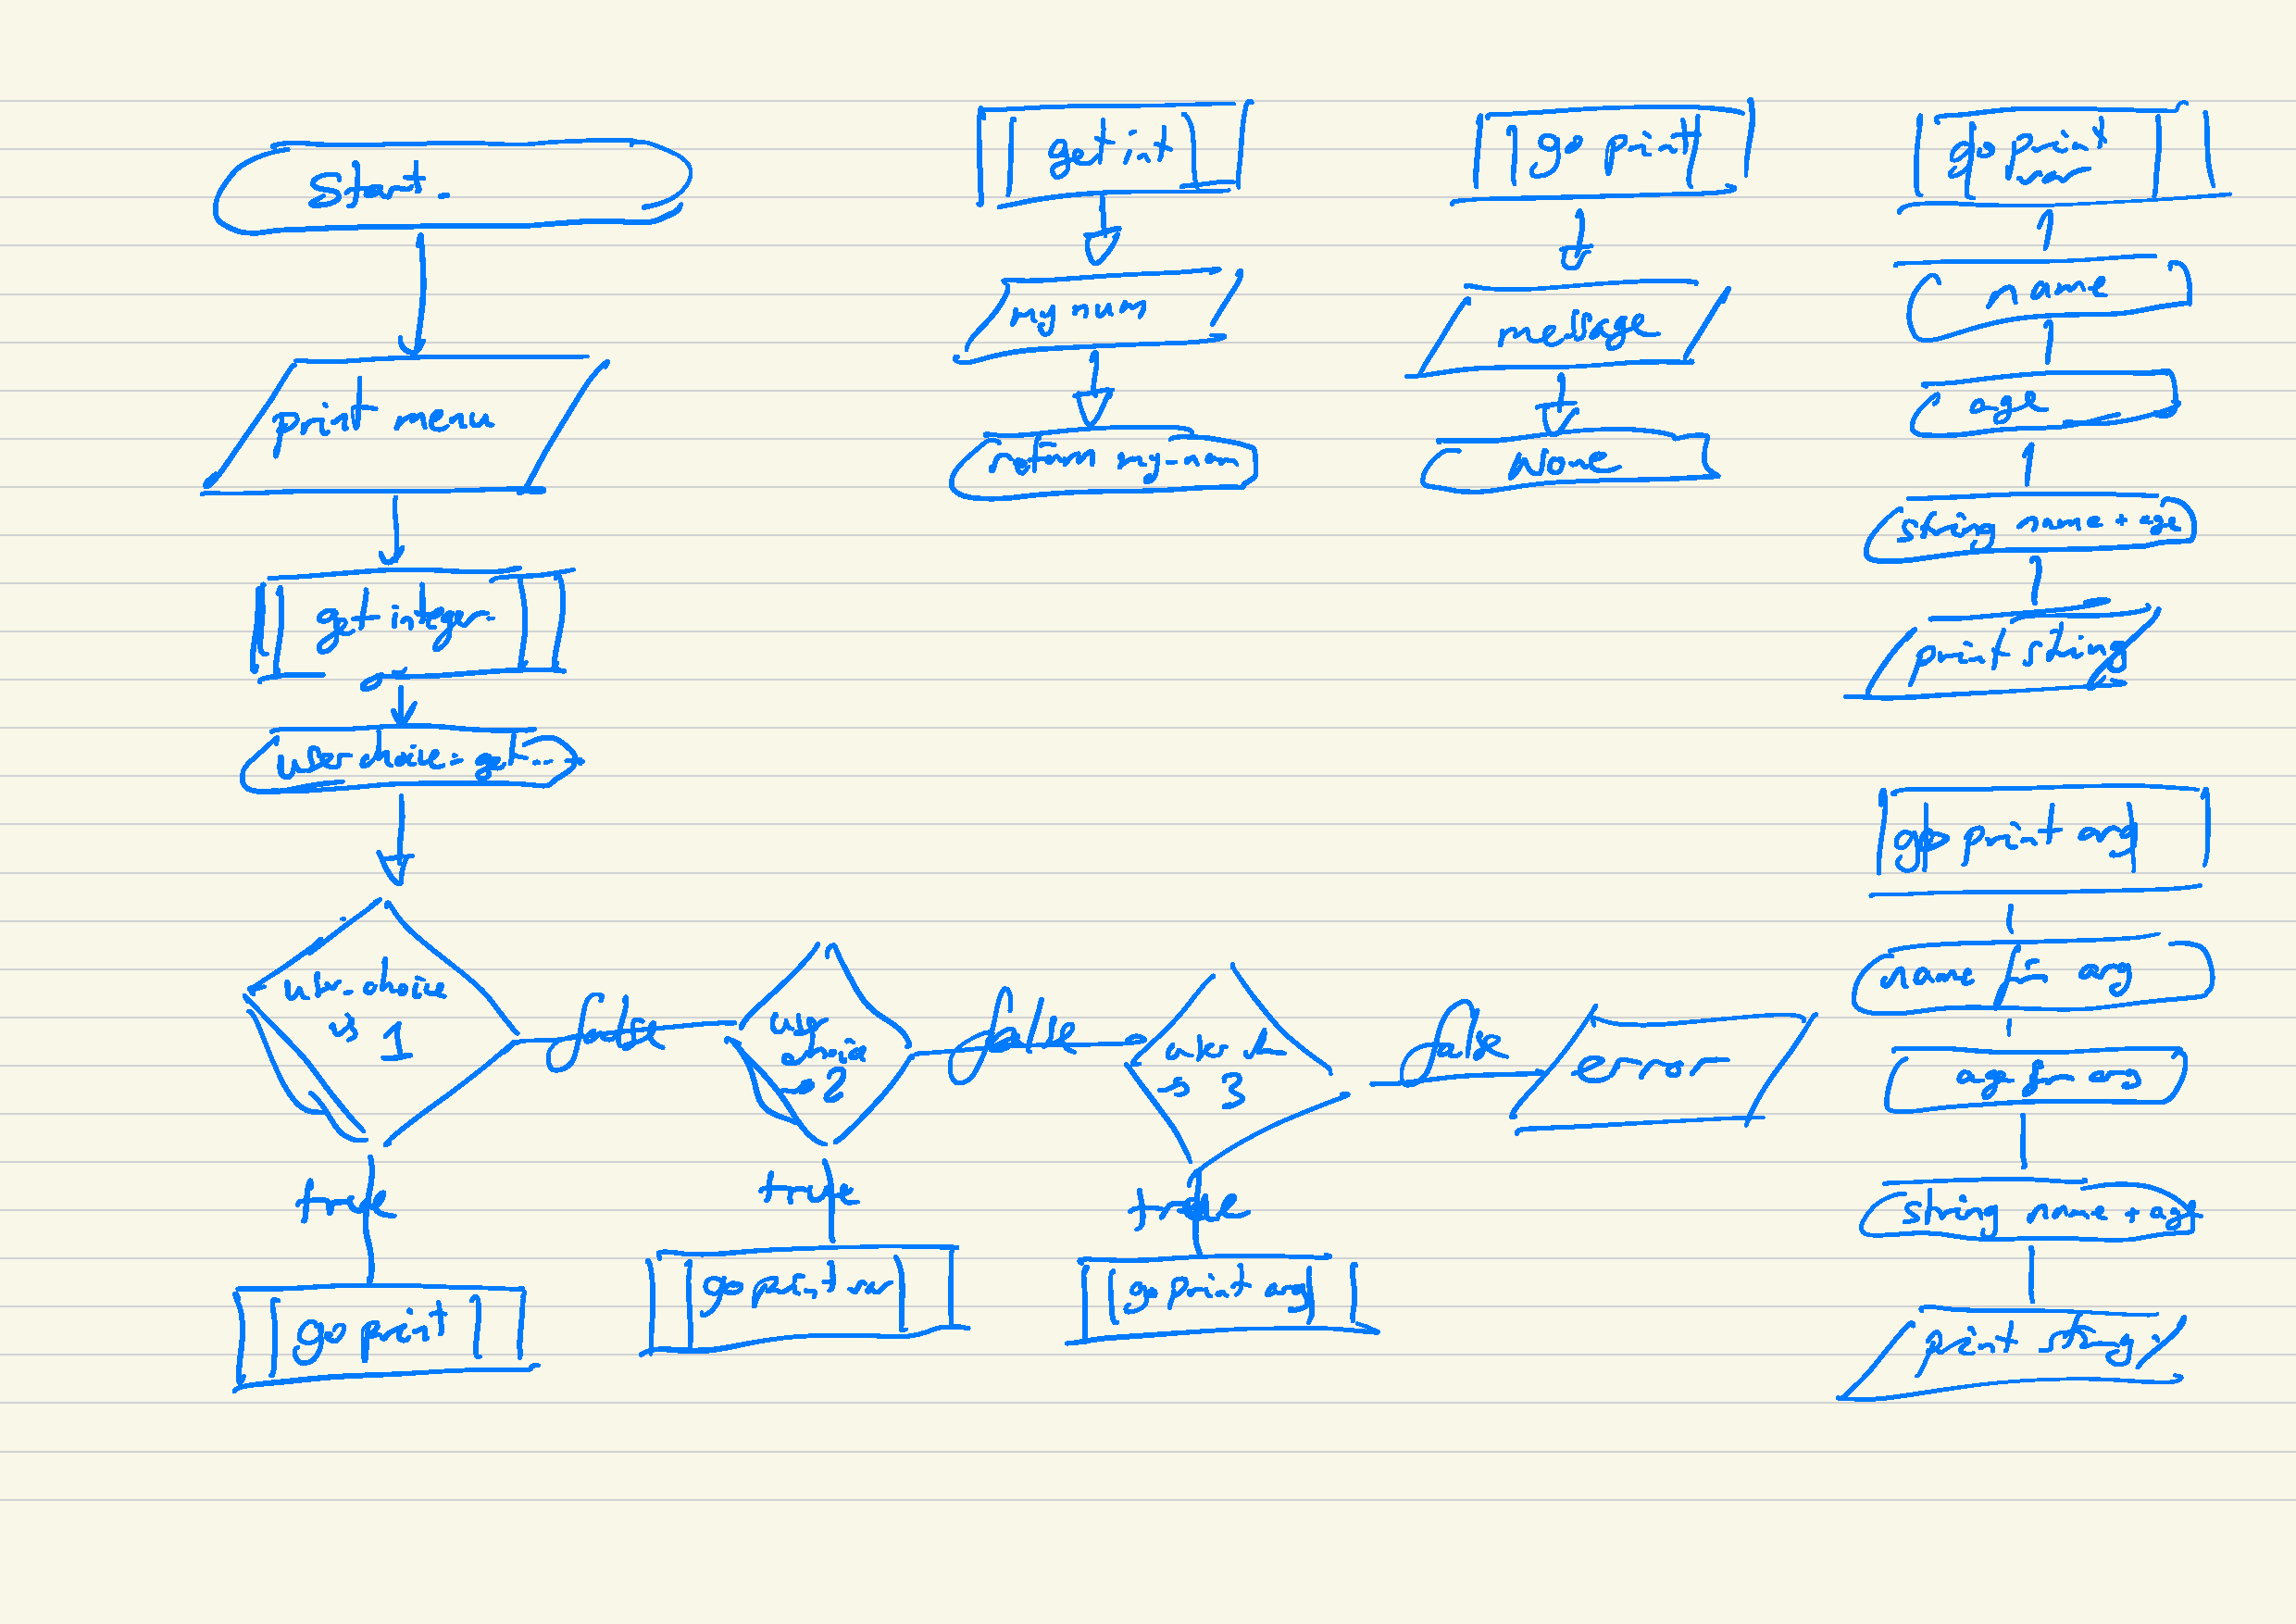
\includegraphics[width=15cm]{function_plan_2_flow_diagram.pdf}
	\caption*{Simple Plan as flow diagram}
\end{figure}

\newpage
\begin{figure}[!ht]
	\centering
	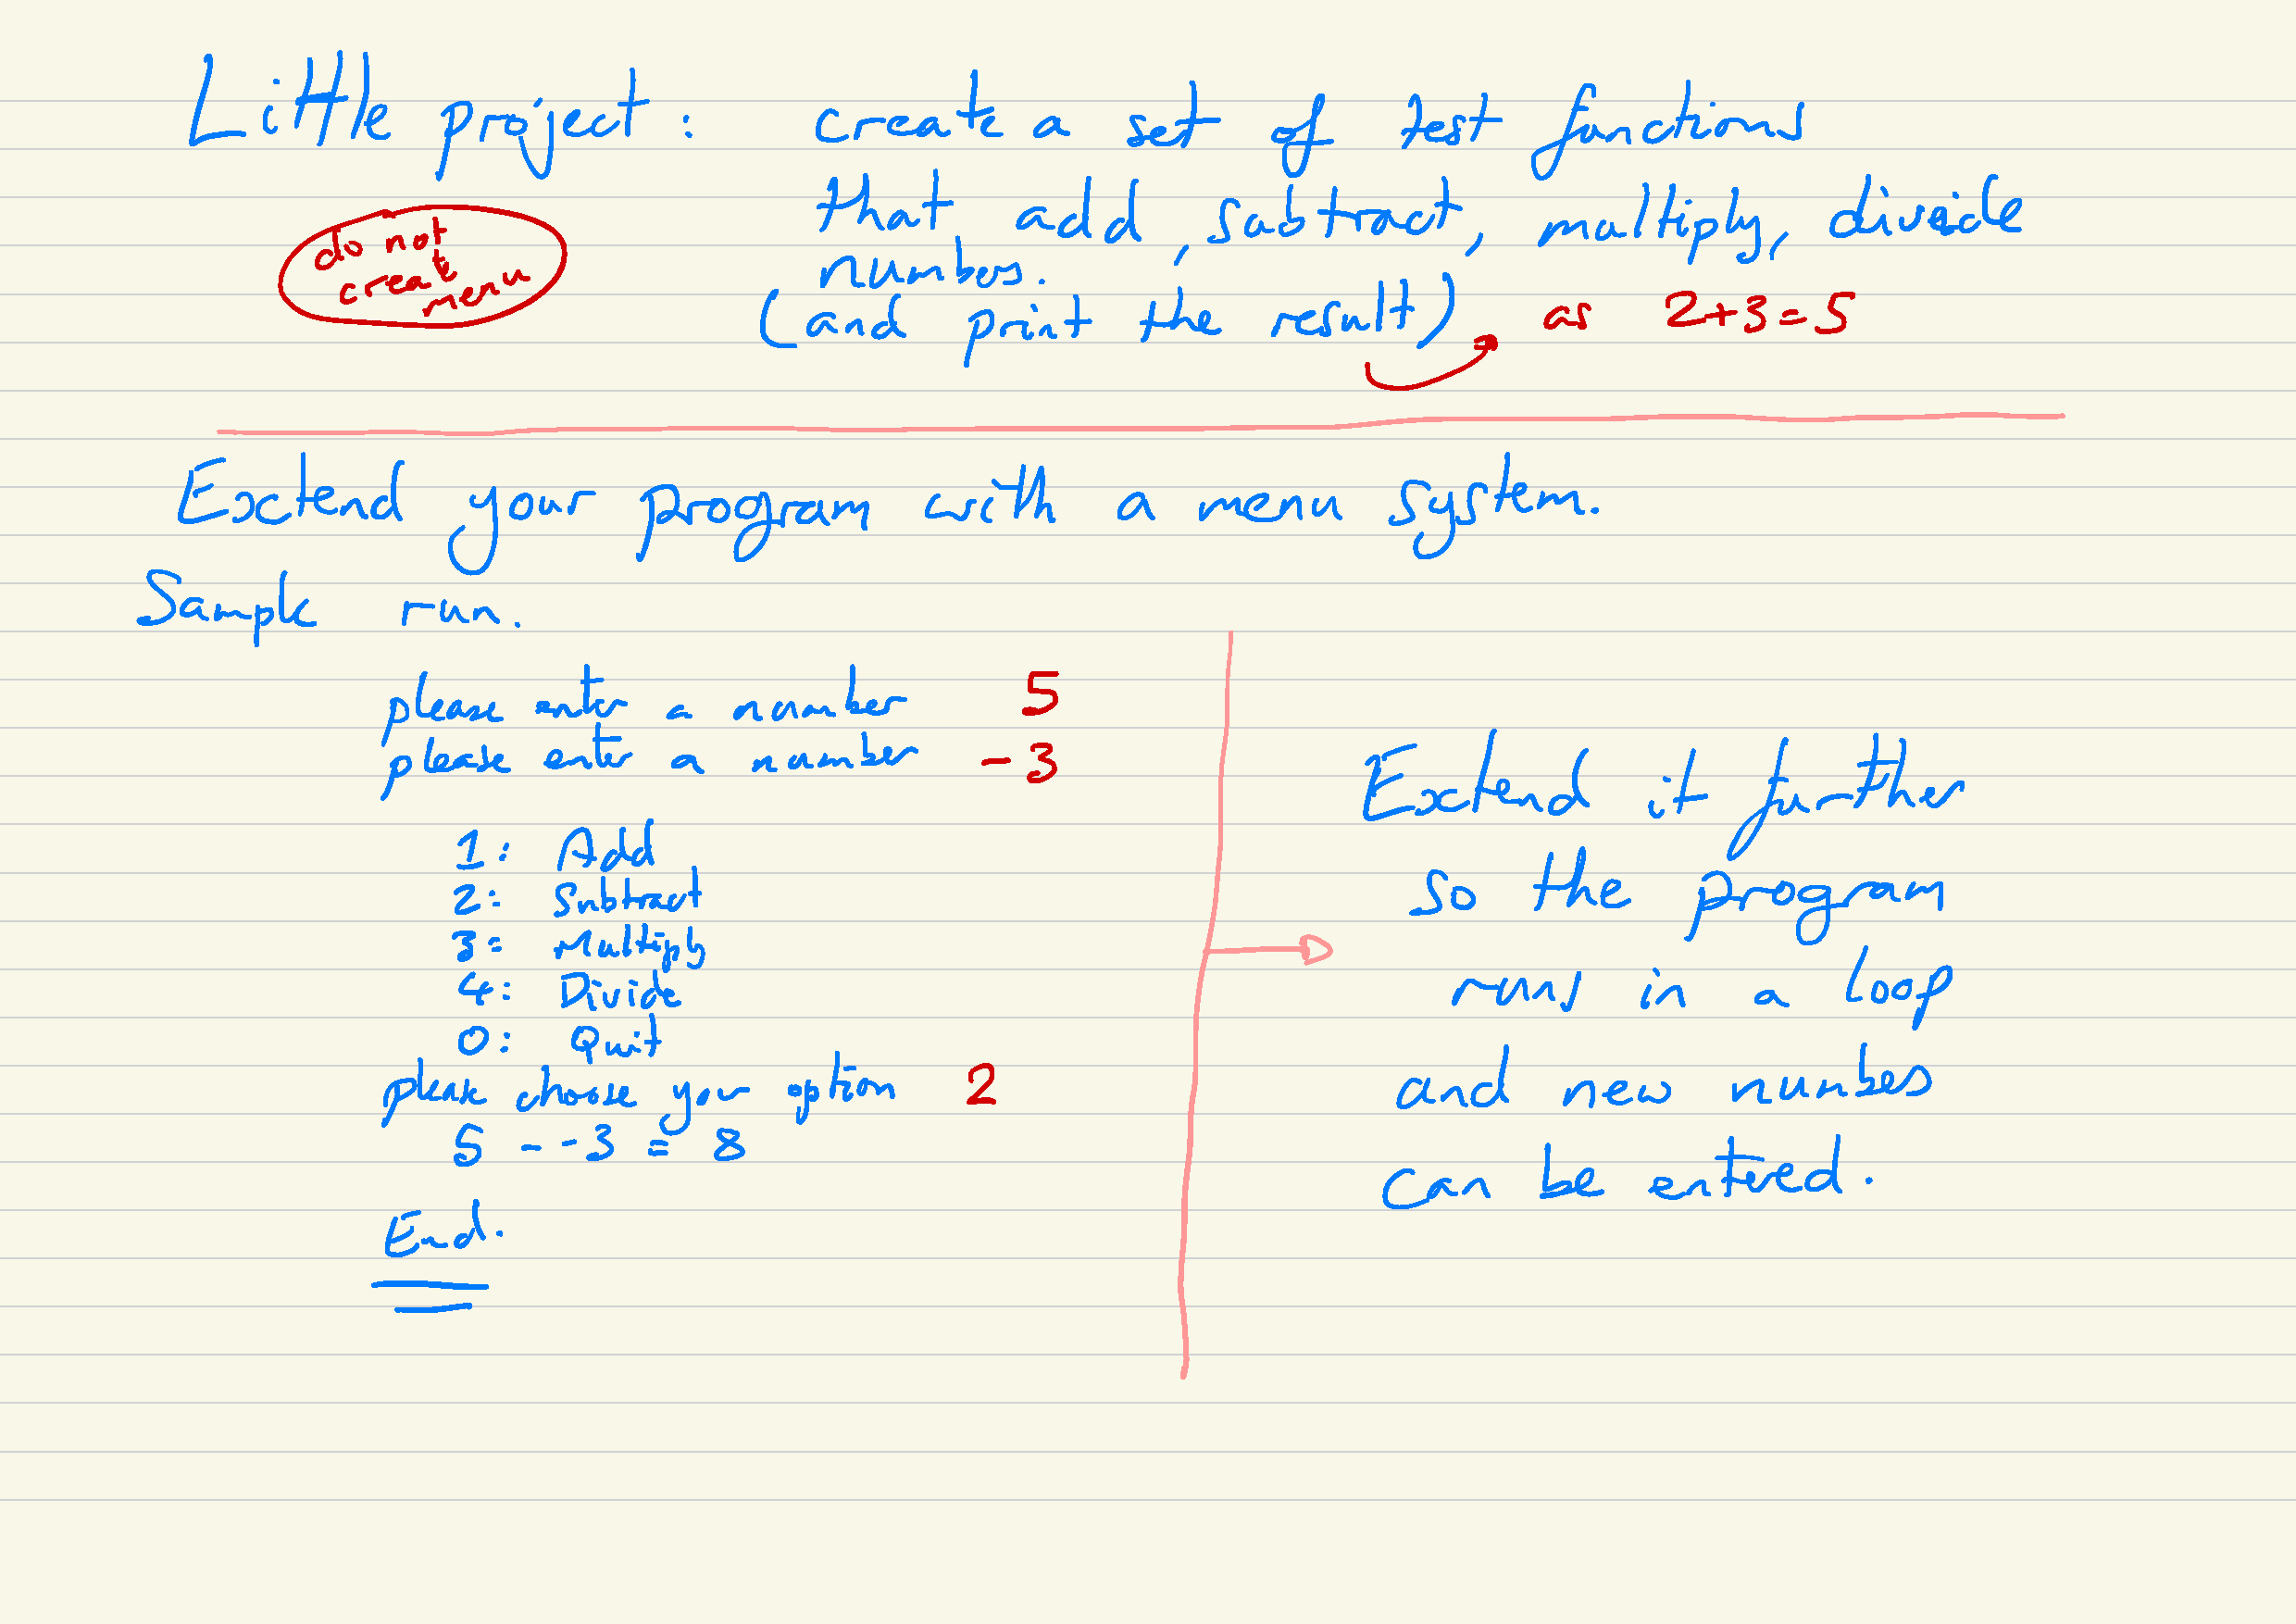
\includegraphics[width=15cm]{little_start_project.pdf}
	\caption*{Little start project}
\end{figure}


\newpage
\section{String Formatting}
Manging strings for print output is critical:\\

Please review using:\\
\url{https://www.w3schools.com/python/python_string_formatting.asp}\\
This means that you actively make variations on the examples given on the page.
\newpage
\section{Loops} 

\begin{figure}[!ht]
	\centering
	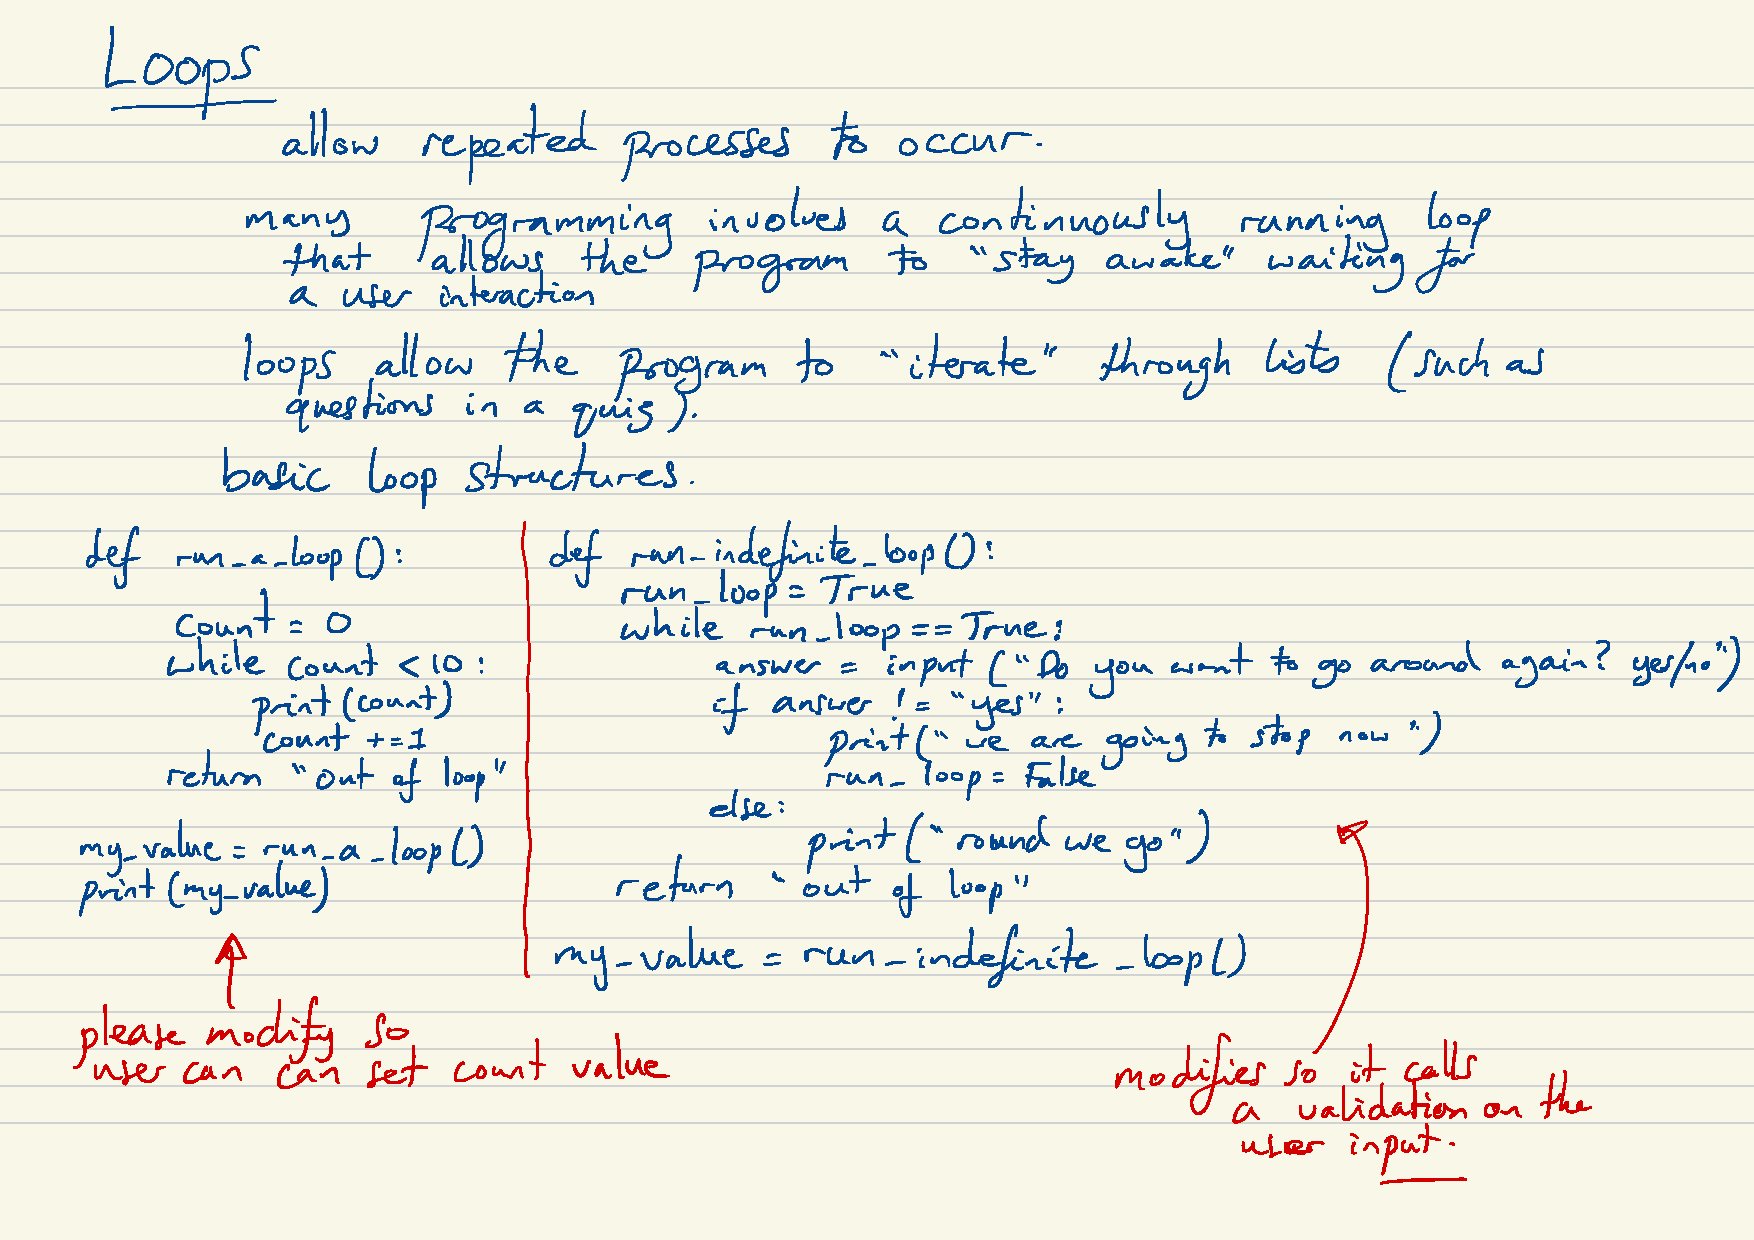
\includegraphics[width=17cm]{loops.pdf}
\end{figure}

\lstinputlisting[language=Python, caption = Test program - functions and menu]{py_files/loops.py}

\newpage
\section{Lists}
Lists are a collection of data items

\begin{figure}[!ht]
	\centering
	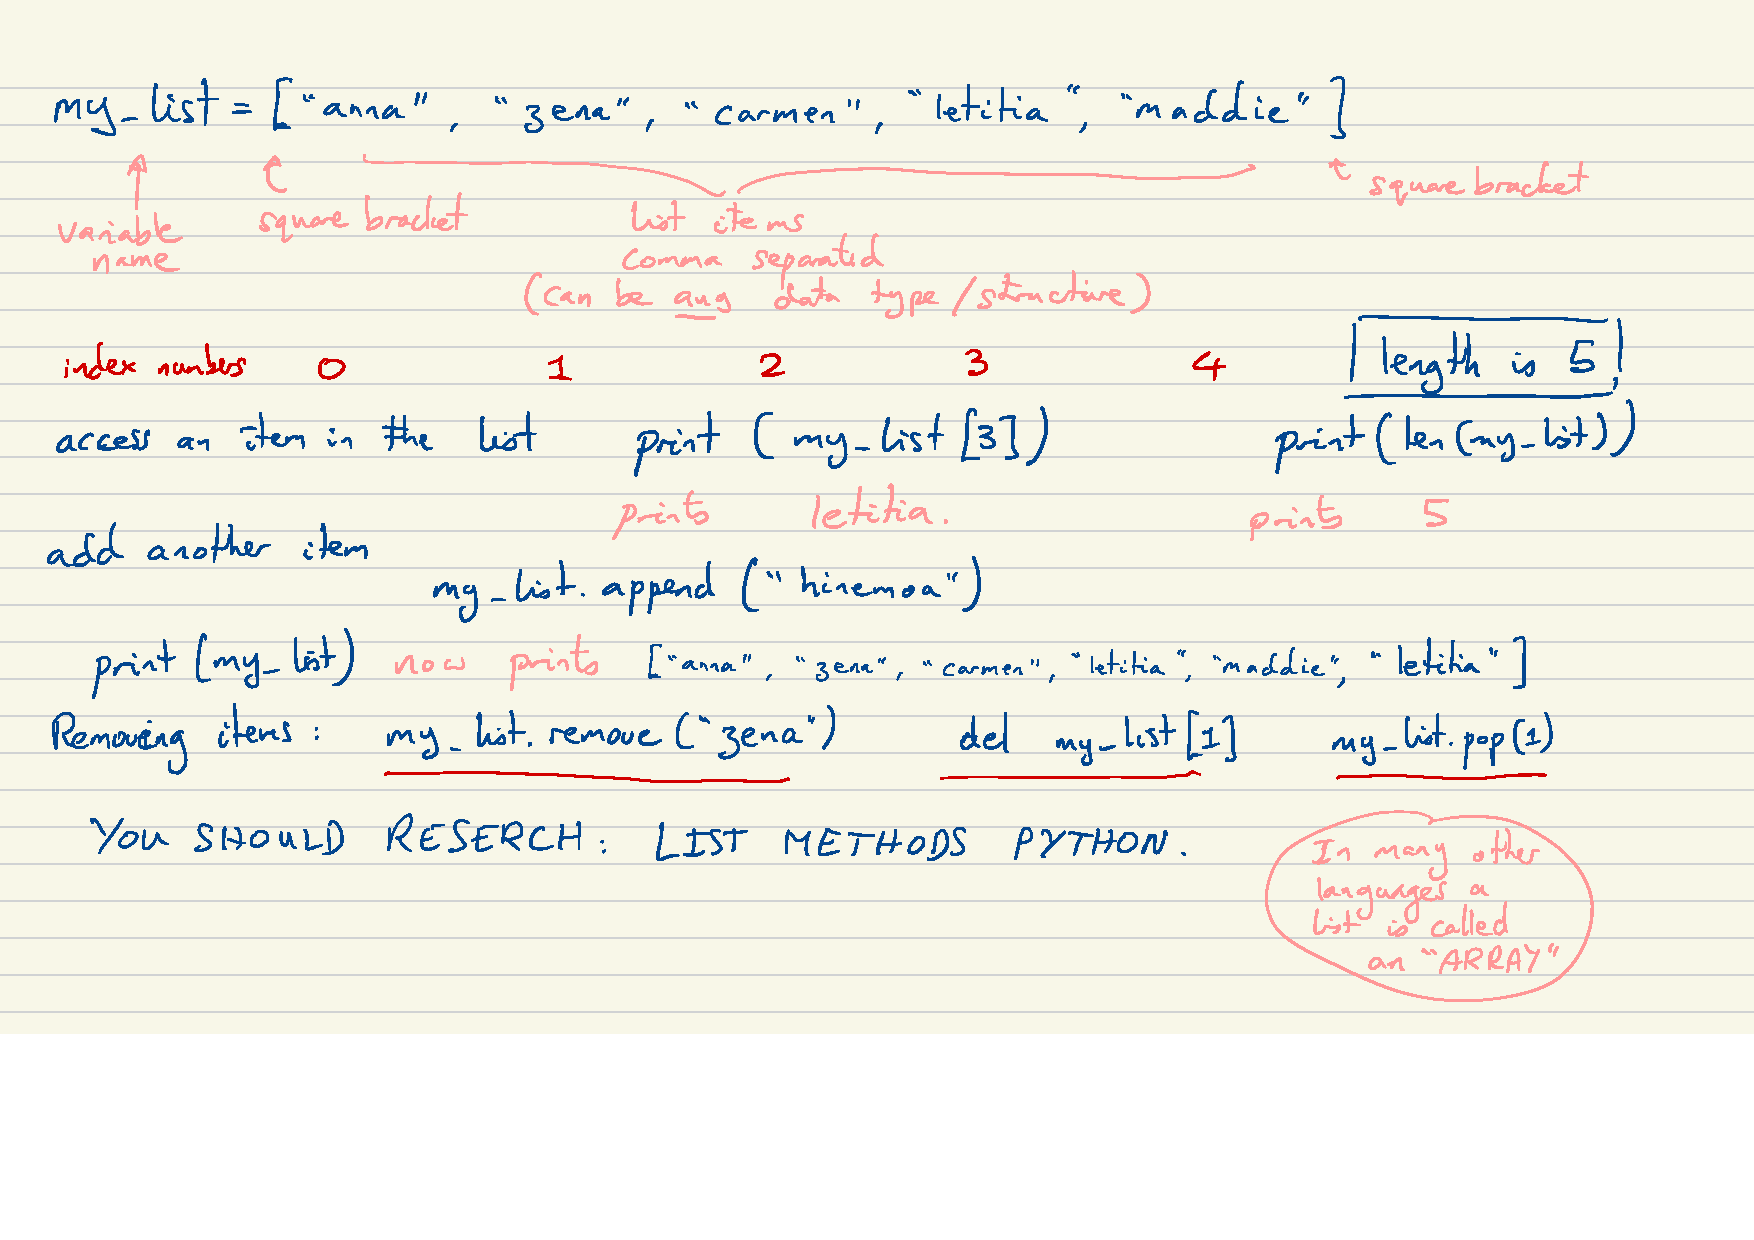
\includegraphics[width=17cm]{lists.pdf}
\end{figure}




\lstinputlisting[language=Python, caption = Lists]{py_files/lists_functions.py}
\subsection{Issues with lists}
\begin{itemize}
	\item The standard error with lists is:  \textbf{IndexError: list index out of range}
\end{itemize}
\subsection{What we should be able to do with lists:}
\begin{itemize}
	\item Create one and access items in the list using index notation.
	\item Find how many items are in the list
	\item Loop through the list and print out items ( have more than one way of doing)
	\item Understand that there are basic \textbf{methods} associated with a list. These mean that we can add, remove, update elements in a list.
\end{itemize}
\subsection{Activities}
\begin{itemize}
	\item Create a function that takes a list as an argument, prints out the list (horizontally), and returns the length of the list
	\item Create a program that asks for the user to enter 5 numbers, it then prints out the sum, average  and product of the numbers (each part is a function).
	\item Create a program that asks for the user to enter 5 numbers, it then prints a menu asking giving users and option to get the sum, product, average of the numbers
\end{itemize}
\section{Validating User Input}
\begin{itemize}
\item Create a function to get input of a single letter from a user.
\item  Create a function to get an integer from a user
\item Create a function to get a string between 2 and 5 letters
\item Create a function to get an integer from a user with boundaries that might change
\end{itemize}
\section{Looping through lists}
\section{Lists with more than one dimension}
Sometimes we wish to store a ``package'' of information.\\
For example , instead of Alice, Bob, Cathy, we might want Alice , Brown, 31 ; Bob Blond 19; Cathy, Black, 21\\
So we have person, hair colour and age.\\

\lstinputlisting[language=Python, caption = Lists]{py_files/multi_structures.py}


\hyperlink{Lists}{This links to a number of code examples}
\newpage
	\hypertarget{Lists}{}
\lstinputlisting[language=Python, caption = Lists]{py_files/lists.py}
\lstinputlisting[caption = Lists]{lists.txt}

\lstinputlisting[language=Python, caption = Menu and Functions]{py_files/menu_list_sums_product_average.py}

\end{document}